\documentclass[12pt]{article}

\usepackage[T3]{fontenc}
\usepackage[utf8]{inputenc}
\usepackage[russian]{babel}

\usepackage{mhchem}
\usepackage{amssymb, amsmath}

\usepackage{tikz}
\usetikzlibrary{shapes.geometric, arrows, positioning, decorations.markings}
\usetikzlibrary{fit}
\usepackage{microtype}
\usepackage{framed}
\usetikzlibrary{decorations.pathmorphing,calc,backgrounds}

\usepackage{animate}

\usepackage{fixltx2e}
\usepackage{hyperref}

%\usetheme{Berkeley}
%\usetheme{Madrid} -- неплохо
%\usetheme{CambridgeUS}
%\usetheme{Singapore}
\usetheme{Warsaw}

\pdfmapfile{+sansmathaccent.map}

\title{Исследование бифуркаций в трехатомных гидридах методом классических траекторий}

\author{\small 
Финенко Артем \\[1ex] 
Научный руководитель: Петров С.В.}

\institute[MSU] % (optional, but mostly needed)
{
  МГУ им. М.В.Ломоносова \\
  Химический факультет
}

\date{23/12/2016}

\pgfdeclareimage[height=0.5cm]{university-logo}{../pictures/logo.jpg}
\logo{\pgfuseimage{university-logo}}

\newcommand\Fontvi{\fontsize{6}{7.2}\selectfont}

\beamertemplatenavigationsymbolsempty

\setbeamerfont{page number in head/foot}{size=\large}
\setbeamertemplate{footline}[frame number]
\setbeamertemplate{frametitle}[default][center]

% change font
\usefonttheme[onlymath]{serif}

% custom block environment
\newenvironment<>{varblock}[2][.9\textwidth]{%
  \setlength{\textwidth}{#1}
  \begin{actionenv}#3%
    \def\insertblocktitle{#2}%
    \par%
    \usebeamertemplate{block begin}}
  {\par%
    \usebeamertemplate{block end}%
  \end{actionenv}}

\tikzstyle{lagrange} = [rectangle, rounded corners, minimum width = 3cm, minimum height = 1cm, text centered, text width = 5cm, draw = black, fill=DarkOrchid!40]

\tikzstyle{equations} = [rectangle, rounded corners, text centered, draw = black, fill=green!30]

\tikzstyle{hamilton} = [rectangle, rounded corners, minimum width = 3cm, minimum height = 1cm, text centered, text width = 5 cm, draw = black, fill = Goldenrod!50]

\tikzstyle{result} = [rectangle, rounded corners, text centered, draw = black, fill = blue!30]

\tikzstyle{arrow} = [thick, ->, >=stealth]

\tikzstyle{vecArrow} = [thick, decoration={markings,mark=at position
   1 with {\arrow[semithick]{open triangle 60}}},
   double distance=1.4pt, shorten >= 5.5pt,
   preaction = {decorate},
   postaction = {draw,line width=1.4pt, white,shorten >= 4.5pt}]

\usepackage{caption}
\usepackage{subcaption}

% theorem environment
\newtheorem{mytheorem}{Теорема}[]

% blackboard symbols
% using dsfont and bbm packages 
\newcommand{\bbA}{\mathds{A}}
\newcommand{\bbI}{\mathds{I}}
\newcommand{\bbB}{\mathds{B}}
\newcommand{\bba}{\mathbbm{a}}
\newcommand{\bbb}{\mathbbm{b}}
\newcommand{\bbS}{\mathds{S}}
\newcommand{\bbE}{\mathds{E}}

% shifting commands
\newcommand{\vlevo}{\hspace*{-0.63cm}}
\newcommand{\vverh}{\vspace*{-0.1cm}}

% round brackets
\newcommand{\lb}{\left(}
\newcommand{\rb}{\right)}

% primes
\newcommand{\dpr}{\prime \prime}

% SKIPS
% "\," -- very small skip

\begin{document}

\begin{titlepage}
\centering
\textbf{\large Московский государственный университет имени М.В.\,Ломоносова\\
\vspace*{0.1cm} Химический факультет\\
\vspace*{0.1cm}
\noindent\makebox[\linewidth]{\rule{\paperwidth}{0.4pt}}
\vspace*{0.1cm}
 Кафедра физической химии\\
\vspace*{0.1cm} Лаборатория строения и квантовой механики молекул \\}
\vspace*{2cm}

\begin{center}
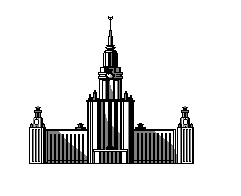
\includegraphics[width=0.3\textwidth]{pictures/logo.jpg}
\end{center}

\vspace*{2cm}
\Large \textbf{Исследование бифуркации в трехатомных гидридах методом классических траекторий.}
\vspace*{2cm}

\begin{flushright}
\large Курсовая работа студента 411 группы\\
Финенко А.А.\\
\vspace{1cm}
Научный руководитель:\\
к.х.н., Петров С.В.
\end{flushright}
\vfill
\large\textbf{Москва\\ 2016}
\end{titlepage}

\tableofcontents

\newpage

\section{Введение}

\section{Схема получения полного колебательно-вращательного гамильтониана}
\subsection{Переход в систему отсчета, связанную с центром масс}

\hspace{0.35cm} Рассмотрим систему $n$ материальных точек. Обозначим их массы через $m_i$, их радиус-векторы в лабораторной системе координат через $\vec{r}_i$, в подвижной системе координат -- через $\vec{R}_i$ ($i = 1 \dots n$). Разделим движение системы на движение центра масс и движение вокруг центра масс:
\vspace*{-0.1cm}
\begin{gather}
\left\{
\begin{aligned}
\vec{r}_1 &= \vec{r} + \vec{r}_1^{\ \prime}, \\
&\cdots \\
\vec{r}_n &= \vec{r} + \vec{r}_n^{\ \prime},
\end{aligned}
\right. \notag
\end{gather}

\hspace*{-0.75cm} где $\vec{r}$ -- радиус-вектор центра масс в лабораторной системе координат и $\vec{r}_i^{\ \prime}$ -- радиус-векторы рассматриваемых точек в системе отсчёта, связанной с центром масс.

Кинетическая энергия $T$ системы принимает вид: 
\vspace*{-0.1cm}
\begin{gather}
T = \frac{1}{2} \sum_{i=1}^{n} m_i \dot{\vec{r}}_i^{\ 2} = \frac{1}{2} \sum_{i=1}^{n} m_i (\dot{\vec{r}} + \dot{\vec{r}}_i^{\ \prime})^2  = \frac{1}{2} M \dot{r}^2 + \frac{1}{2} \sum_{i=1}^{n} m_i ( \dot{r}_i^\prime)^2 + \dot{\vec{r}} \sum_{i=1}^{n} m_i \dot{\vec{r}}_i^{\ \prime}, \notag
\end{gather}

\hspace*{-0.75cm} где $M = \sum_{i=1}^{n} m_i$.

Заметим, что последняя сумма является производной следующей суммы, которая равна нулю: 
\vspace*{-0.1cm}
\begin{gather}
\sum_{i=1}^{n} m_i \dot{\vec{r}}_i^{\ \prime} = \frac{d}{dt} \sum_{i=1}^{n} m_i \vec{r}_i^{\ \prime} = 0. \notag
\end{gather}

Итак, мы перешли в систему координат, связанную с центром масс, и отделили энергию движения центра масс:
\vspace*{-0.1cm}
\begin{gather}
T = \frac{1}{2} M \dot{r}^2 + \frac{1}{2} \sum_{i=1}^{n} m_i( \dot{r}_i^\prime)^2. \notag
\end{gather}

Забудем про слагаемое, отвечающее центру масс; откинем штрихи, чтобы упростить запись.

\subsection{Переход в подвижную систему отсчета}

Переход от лабораторной системы отсчета к подвижной системе может быть осуществлен при помощи трех последовательных поворотов на углы Эйлера $\varphi$, $\theta$ и $\psi$. 

\begin{figure}
  \centering
	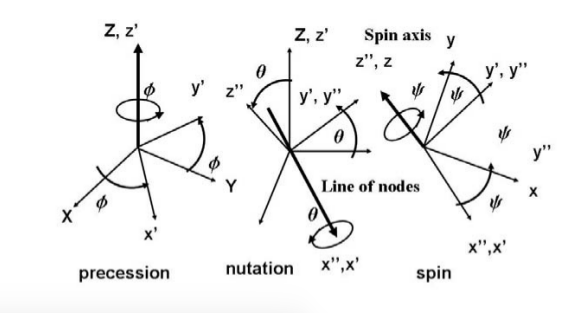
\includegraphics[width=0.7\textwidth]{pictures/EulerAngles.jpg}
	\caption{Углы Эйлера}
	\label{fig:EulerAngles}
\end{figure}

Первое вращение происходит вокруг оси $z$ на угол $\varphi$. Оно переводит лабораторную систему $x, y, z$ в систему $x^\prime$, $y^\prime$, $z^\prime$. Угол $\varphi$ называется углом прецессии.
\begin{gather}
\begin{pmatrix}
x^\prime \\
y^\prime \\
z^\prime
\end{pmatrix} = 
\begin{pmatrix}
\cos \varphi & \sin \varphi & 0 \\
- sin \varphi & \cos \varphi & 0 \\
0 & 0 & 1
\end{pmatrix}
\begin{pmatrix}
x \\
y \\
z
\end{pmatrix} =
\bbS_\varphi
\begin{pmatrix}
x \\
y \\
z
\end{pmatrix} \notag
\end{gather}

Оси  $x^\prime$, $y^\prime$ лежат в плоскости $x$, $y$. Затем происходит поворот вокруг оси $x^\prime$ на угол $\theta$, переводящий систему $x^\prime$, $y^\prime$, $z^\prime$ в систему $x^{\dpr}$, $y^{\dpr}$, $z^{\dpr}$. Ось $x^{\dpr}$ совпадает с осью $x^{\prime}$. Ось этого поворота называется линией узлов. Угол $\theta$ называется углом нутации.

\begin{gather}
\begin{pmatrix}
x^{\dpr} \\
y^{\dpr} \\
z^{\dpr} 
\end{pmatrix} = 
\begin{pmatrix}
1 & 0 & 0 \\
0 & \cos \theta & \sin \theta \\
0 & - sin \theta & \cos \theta
\end{pmatrix}
\begin{pmatrix}
x^\prime \\
y^\prime \\
z^\prime
\end{pmatrix} = 
\bbS_\theta
\begin{pmatrix}
x^\prime \\
y^\prime \\
z^\prime
\end{pmatrix} \notag
\end{gather}   

И наконец, вращение вокруг оси $z^{\dpr}$ на угол $\psi$ переводит систему $x^{\dpr}$, $y^{\dpr}$, $z^{\dpr}$ в систему $x$, $y$, $z$. Угол $\psi$ называется углом собственного вращения.

\begin{gather}
\begin{pmatrix}
X \\
Y \\
Z
\end{pmatrix} =
\begin{pmatrix}
\cos \psi & \sin \psi & 0 \\
- \sin \psi & \cos \psi & 0 \\
0 & 0 & 1
\end{pmatrix}
\begin{pmatrix}
x^{\dpr} \\
y^{\dpr} \\
z^{\dpr}
\end{pmatrix} = 
\bbS_\psi 
\begin{pmatrix}
x^{\dpr} \\
y^{\dpr} \\
z^{\dpr}
\end{pmatrix} \notag
\end{gather}

Суммарное вращение представляет собой последовательное применение описанных поворотов и имеет следующую матрицу: 
\begin{gather}
\begin{pmatrix}
X \\
Y \\
Z
\end{pmatrix} = 
\bbS 
\begin{pmatrix}
x \\
y \\
z
\end{pmatrix} \notag \\
\bbS = \bbS_\psi \bbS_\theta \bbS_\varphi = 
\begin{pmatrix}
\cos \psi \cos \varphi - \cos \theta \sin \varphi \sin \psi & \cos \psi \sin \varphi + \cos \theta \cos \varphi \sin \psi & \sin \theta \sin \psi \\
- \sin \psi \cos \varphi - \cos \theta \sin \varphi \cos \psi & - \sin \psi \sin \varphi + \cos \theta \cos \varphi \cos \psi & \sin \theta \cos \psi \\
\sin \psi \sin \theta & - \cos \varphi \sin \theta & \cos \theta 
\end{pmatrix} \notag
\end{gather}

Проектируя вектор угловой скорости $\Omega$ на базис, образованный Эйлеровыми угловыми скоростями $\dot{\varphi}$, $\dot{\theta}$, $\dot{\psi}$, получаем соотношение, известное как кинематическое уравнение Эйлера:

\begin{gather}
\begin{pmatrix}
\Omega_X \\
\Omega_Y \\
\Omega_Z
\end{pmatrix} =
\begin{pmatrix}
\sin \theta \sin \psi & \cos \psi & 0 \\
\sin \theta \cos \psi & - \sin \psi & 0 \\
\cos \theta & 0 & 1
\end{pmatrix}
\begin{pmatrix}
\dot{\varphi} \\
\dot{\theta} \\
\dot{\psi}
\end{pmatrix} \notag
\end{gather}

\begin{figure}
  \centering
	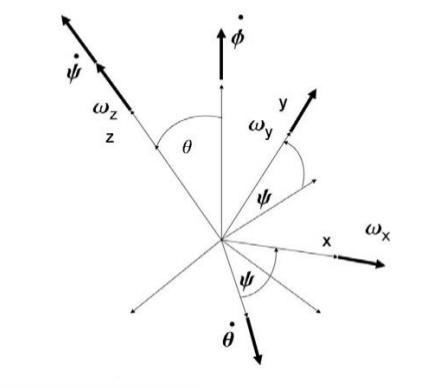
\includegraphics[width=0.5\textwidth]{pictures/AngularVelocities.jpg}
	\caption{Угловые скорости}
	\label{fig:AngularVelocities}
\end{figure}

ПОПРАВИТЬ НА КАРТИНКЕ МАЛЕНЬКИЕ БУКВЫ НА БОЛЬШИЕ

Я НЕ ЗНАЮ КАК СВЯЗАТЬ НАПИСАННОЕ НИЖЕ С ТЕМ, ЧТО ДОПИСАНО СЕЙЧАС

Перейдём в подвижную систему координат при помощи ортогональной матрицы $\bbS$:
\vspace*{-0.1cm}
\begin{gather}
\vec{r}_i = \bbS \vec{R}_i, \quad i = 1 \dots n. \notag
\end{gather}

Введем матрицу $\bbA$ следующим образом: $\bbA = \dot{\bbS} \bbS^{-1}$. Покажем, что она является кососимметрической матрицей; для этого продифференцируем единичную матрицу:
\vspace*{-0.1cm}
\begin{gather}
\frac{d}{dt} \bbE = \frac{d}{dt} \left( \bbS \bbS^{-1}\right) = \dot{\bbS} \bbS^{-1} + \bbS \dot{\bbS}^{-1} = 0. \notag
\end{gather}

Заметим, что первое слагаемое и есть матрица $\bbA$, а второе -- транспонированная матрица $\bbA$ (т.к. $\bbS^\top = \bbS^{-1}$ в силу ортогональности). Следовательно,
\vspace*{-0.1cm}
\begin{gather}
\bbA + \bbA^\top = 0, \notag
\end{gather}

\hspace*{-0.75cm} т.е. по определению матрица $\bbA$ является кососимметрической.

Так как размерность пространства кососимметрических матриц равна 3, то существует естественный изоморфизм, позволяющий сопоставить каждой кососимметрической матрице единственный псевдовектор:
\vspace*{-0.1cm}
\begin{gather}
\bbA = 
\begin{pmatrix}
0 & -\omega_3 & \omega_2 \\
\omega_3 & 0 & -\omega_1 \\
-\omega_2 & \omega_1 & 0
\end{pmatrix}
\quad
\longleftrightarrow
\quad
\vec{\omega} = 
\begin{pmatrix}
\omega_1 \\
\omega_2 \\
\omega_3
\end{pmatrix}
,
\notag
\end{gather}

\hspace*{-0.75cm} причем для любого вектора $\vec{x} \in \mathbf{R}^3$ имеем $\bbA \vec{x} = [ \vec{\omega} \times \vec{x} ]$, где $\vec{\omega}$ -- вектор угловой скорости в лабораторной системе координат.

Получим выражение для квадратов скоростей рассматриваемых точек в лабораторной системе координат через координаты и скорости в подвижной системе координат:
\vspace*{-0.1cm}
\begin{gather}
\dot{\vec{r}}_i = \bbS \dot{\vec{R}}_i + \dot{\bbS} \vec{R}_i = \dot{\bbS} \bbS^{-1} \vec{r}_i + \bbS \dot{\vec{R}}_i  = \bbA \vec{r}_i + \bbS \dot{\vec{R}}_i = [ \vec{\omega} \times \vec{r}_i ] + \bbS \dot{\vec{R}}_i = [\bbS \vec{\Omega} \times \bbS \vec{R}_i ] + \bbS \dot{\vec{R}}_i = \notag \\
= \bbS \left( [\vec{\Omega} \times \vec{R}_i ] + \dot{\vec{R}}_i \right)  \notag , \\
\dot{r}_i^2 = \dot{\vec{r}}_i^{\ \top} \dot{\vec{r}}_i = \left( \dot{\vec{R}}_i + [ \vec{\Omega} \times \vec{R}_i] \right)^\top \bbS^\top \bbS \left( \dot{\vec{R}}_i + [ \vec{\Omega} \times \vec{R}_i ] \right) = \dot{R}_i^2 + 2 \dot{\vec{R}}_i \ [ \vec{\Omega} \times \vec{R}_i] + [ \vec{\Omega} \times \vec{R}_i ]^2 \notag ,
\end{gather}

\hspace*{-0.75cm} где $\vec{\Omega}$ -- вектор угловой скорости в подвижной системе координат.

Рассмотрим последнее слагаемое как смешанное произведение и применим правило Лагранжа:
\vspace*{-0.1cm}
\begin{gather}
([\vec{\Omega} \times \vec{R}_i] , [\vec{\Omega} \times \vec{R}_i]) = \vec{\Omega}^\top [ \vec{R}_i \times [ \vec{\Omega} \times \vec{R}_i ]] = \vec{\Omega}^\top \left( \vec{\Omega} (\vec{R}_i, \vec{R}_i ) - \vec{R}_i (\vec{R}_i, \vec{\Omega} ) \right)
\notag .
\end{gather}

Итак, с учётом выполненных преобразований имеем:
\vspace*{-0.1cm}
\begin{gather}
T = \frac{1}{2} \sum_{i=1}^{n} m_i \dot{r}_i^2 = \frac{1}{2} \sum_{i=1}^{n} m_i \dot{R}_i^2 + \vec{\Omega} ^\top \sum_{i=1}^{n} m_i[ \vec{R}_i \times \dot{\vec{R}}_i ] + \frac{1}{2} \vec{\Omega}^\top \sum_{i=1}^{n} m_i \left( \vec{\Omega} (\vec{R}_i, \vec{R}_i ) - \vec{R}_i (\vec{R}_i, \vec{\Omega} ) \right) = 
\notag \\
= \frac{1}{2} \sum_{i=1}^{n} m_i \dot{R}_i^2 + \vec{\Omega}^\top \sum_{i=1}^{n} m_i [ \vec{R}_i \times \dot{\vec{R}}_i ] + \vec{\Omega}^\top \mathbb{I} \ \vec{\Omega} \notag .
\end{gather}

\vlevo где $\bbI$ -- матрица тензора инерции в подвижной системе координат.

Пусть исследуемая система содержит $s$ внутренних степеней свободы. Осуществим переход от векторов в подвижной системе к внутренним координатам $q_j, j=1 \dots s$:
\vverh
\begin{gather}
\left\{
\begin{aligned}
\vec{R}_1 &= \vec{R}_1 (q_1, \dots, q_s), \\
&\cdots \\
\vec{R}_n &= \vec{R}_n (q_1, \dots, q_s);
\end{aligned}
\right. \notag \\
\frac{d}{dt} \vec{R}_i = \sum_{j=1}^{s} \frac{\partial \vec{R}_i}{\partial q_j} \ \dot{q}_j \notag .
\end{gather}

Подставляя $\dot{\vec{R}}_i$ в выражение для кинетической энергии, получим:
\vverh
\begin{gather}
T = \frac{1}{2} \sum_{i=1}^{n} m_i \sum_{j=1}^{s} \frac{\partial \vec{R}_i}{\partial q_j} \dot{q}_j \sum_{k=1}^{s} \frac{\partial \vec{R}_i}{\partial q_k} \dot{q}_k + \vec{\Omega}^\top \sum_{i=1}^{n} m_i \left[ \vec{R}_i \times \sum_{j=1}^{s} \frac{\partial \vec{R}_i}{\partial q_j} \ \dot{q}_j \right] + \vec{\Omega}^\top \bbI \ \vec{\Omega} = \notag \\
= \frac{1}{2} \sum_{j=1}^{s} \sum_{k=1}^{s} \left( \sum_{i=1}^{n} m_i \frac{\partial \vec{R}_i}{\partial q_j} \frac{\partial \vec{R}_i}{\partial q_k} \right) \dot{q}_j \dot{q}_k + \vec{\Omega}^\top \sum_{j=1}^{s} \left( \sum_{i=1}^{n} m_i \left[ \vec{R}_i \times \frac{\partial \vec{R}_i}{\partial q_j} \right] \right) \dot{q}_j + \frac{1}{2} \vec{\Omega}^\top \bbI \ \vec{\Omega} \notag .
\end{gather}

Обозначая $a_{jk} = \sum_{i=1}^{n} m_i \frac{\partial \vec{R}_i}{\partial q_j} \frac{\partial \vec{R}_i}{\partial q_k}$, $A_{jk} = \sum_{i=1}^{n} m_i \left[ \vec{R}_i \times \frac{\partial \vec{R}_i}{\partial q_k} \right]_{\alpha}$ (здесь $\alpha = x,y,z$ соответствуют $j=1,2,3$), представим кинетическую энергию в виде:
\vverh
\begin{gather}
T = \frac{1}{2} \dot{\vec{q}}^{\, \top} \bba \ \dot{\vec{q}} + \vec{\Omega}^\top \bbA \ \dot{\vec{q}} + \frac{1}{2} \vec{\Omega}^\top \bbI \ \vec{\Omega} \notag ,
\end{gather}

\vlevo где $\bba = (a_{jk})_{j=1 \dots s, \ k=1 \dots s}$, $\bbA = (A_{jk})_{j=1 \dots 3, \ k=1 \dots s}$.

\subsection{Применение теоремы Донкина}
Перепишем выражение для кинетической энергии в матричном виде для того, чтобы перейти к гамильтоновым переменным.
\begin{gather}
T = \frac{1}{2} 
\begin{bmatrix}
\vec{\Omega}^{\top} \ \dot{\vec{q}}^{\, \top}
\end{bmatrix}
\bbB
\begin{bmatrix}
\vec{\Omega} \\
\dot{\vec{q}}
\end{bmatrix}, \notag
\end{gather}

где $\bbB$ -- блочная матрица:
\begin{gather}
\bbB = 
\begin{bmatrix}
\bbI & \bbA \\
\bbA^\top & \bba
\end{bmatrix} \notag
\end{gather}  

\tikzstyle{arrow} = [thick, ->, >=stealth]
\tikzstyle{vecArrow} = [thick, decoration={markings,mark=at position
   1 with {\arrow[semithick]{open triangle 60}}},
   double distance=1.4pt, shorten >= 5.5pt,
   preaction = {decorate},
   postaction = {draw,line width=1.4pt, white,shorten >= 4.5pt}]

\tikzstyle{lagrange} = [rectangle, rounded corners, minimum width = 3cm, minimum height = 1cm, text centered, text width = 7cm, draw = black, fill=red!30]

\tikzstyle{hamilton} = [rectangle, rounded corners, minimum width = 3cm, minimum height = 1cm, text centered, text width = 7cm, draw = black, fill=yellow!30]

\tikzstyle{equations} = [rectangle, rounded corners, minimum width = 3cm, minimum height = 1cm, text centered, text width = 5cm, draw = black, fill=green!30]
    
\begin{tikzpicture}[node distance = 2cm, auto]

\node (lag1) [lagrange] {$\mathcal{L} = \mathcal{L}(\vec{q}, \dot{\vec{q}})$};

\node (ham1) [hamilton, right = 2 cm of lag1] {$\mathcal{H} = \mathcal{H}(\vec{q}, \vec{p})$};

\node (eq1) [equations, below = 0.5 cm of lag1] {$\vec{p} = \frac{\partial \mathcal{L}}{\partial \dot{\vec{q}}}$};

\node (eq2) [equations, below = 0.5 cm of ham1] {$\dot{\vec{q}} = \frac{\partial \mathcal{L}}{\partial \vec{p}}$};

\node (lag2) [lagrange, below = 2 cm of lag1] {$\mathcal{L} = \mathcal{L}(\vec{\Omega})$};

\node (ham2) [hamilton, below = 2 cm of ham1] {$\mathcal{H} = \mathcal{H} (\vec{J})$};

\node (eq3) [equations, below = 0.5 cm of lag2] {$\vec{J} = \frac{\partial \mathcal{L}}{\partial \vec{\Omega}}$};

\node (eq4) [equations, below = 0.5 cm of ham2] {$\vec{\Omega} = \frac{\partial \mathcal{H}}{\partial \vec{J}}$};

\draw [vecArrow] (lag1) -- (ham1);

\draw [vecArrow] (lag2) -- (ham2);

\end{tikzpicture}



\newpage

% modifying font of the appendix title
\appendix
\titleformat{\chapter}[display]
  {\normalfont\large\bfseries}% <- font for label "Appendix A", default \huge
  {\chaptertitlename\ \thechapter}
  {20pt}
  {\large}

\section{Про угловой момент..}
  
Покажем истинность следующего результата:
\begin{gather}
\vec{J} = \bbA \dot{\vec{q}} + \bbI \, \vec{\Omega} \notag
\end{gather}

Рассмотрим угловой момент в лабораторной системе координат.

\begin{gather}
\vec{j} = \sum_{i=1}^{n} m_i \left[ \vec{r}_i \times \dot{\vec{r}}_i \right] \notag \\
\dot{\vec{r}}_i = \bbS^{-1} \lb \left[ \vec{\Omega} \times \vec{R}_i \right] + \dot{\vec{R}}_i \rb \notag \\
\vec{j} = \sum_{i=1}^{n} m_i \left[ \vec{r}_i \times \bbS^{-1} \lb \left[ \vec{\Omega} \times \vec{R}_i \right] + \dot{\vec{R}}_i \rb \right] =
\bbS^{-1} \sum_i m_i \left[ \vec{R}_i \times \dot{\vec{R}}_i \right] + \bbS^{-1} \sum_i m_i \left[ \vec{R}_i \times \left[ \vec{\Omega} \times \vec{R}_i \right] \right] \notag
\end{gather}

Внимательно посмотрим на слагаемое, содержащее двойное векторное произведение:
\begin{gather}
\sum_i m_i \left[ \vec{R}_i \times \left[ \vec{\Omega} \times \vec{R}_i \right] \right] = \sum_i \lb R_i^2 \vec{\Omega} - \lb \vec{R}_i , \vec{\Omega} \rb \vec{R}_i \rb = \bbI \vec{\Omega} \notag
\end{gather}

Используем результат, умножаем обе части на $\bbS$, учтем, что $\vec{J} = \bbS \vec{j}$: 
\begin{gather}
\vec{J} = \bbA \dot{\vec{q}} + \bbI \, \vec{\Omega} \notag 
\end{gather}

Что-то другое

Какая-нибудь фигня

какая-нибудь ересь

штото

\end{document}